\chapter{Test}
\label{chap:test}

\section{Aufgabenverteilung}

Wir haben die folgende Verteilung beschlossen:\\

\textbf{Testleiter:} Tobias Kerst

Kümmert sich darum, den Test zu erklären und geht die einzelnen Aufgaben mit dem Probanden durch.

\textbf{Unterstützung Testleiter/Interaktionsmanagement:} Maike Rees

Ist für die einzelnen Screens zuständig, dass beim Klicken auf klickbare Elemente die entsprechenden Fenster und Dialoge aufgehen.

\textbf{Protokollant:} Patrick König

Ist für die Dokumentation des Tests zuständig. Hierbei wird der Test an sich und die Nachbesprechung festgehalten.

\section{Testvorbesprechungs-Anleitung}
\label{sec:testvorbesprechung}

Die hier genannten Punkte sind die Anweisungen für den Testleiter, wie er den Probanden auf den Test vorbereiten soll. Der Testleiter probiert diese Punkte in einer lockeren Atmosphäre zu erläutern.

\begin{itemize}
\item Dem Probanden muss klargemacht werden, dass nicht er, sondern nur unsere App getestet wird. Dabei soll uns der Proband helfen.

\item Sage dem Probanden, dass wir versuchen, Fehler an der grafischen Oberfläche zu erkennen.

\item Er soll versuchen, sich diese zu merken, wenn ihm etwas komisch vorkommt oder bestimmte Dinge nicht gefunden werden. Wir sind für jeden gefundenen Fehler an der App dankbar.

\item Erkläre dem Teilnehmer, dass er sich bei dem Test so viel Zeit lassen kann, wie er möchte.

\item Erkläre dem Teilnehmer, dass es vollkommen in Ordnung ist, den Test abzubrechen oder eine kleine Pause einzulegen, wenn er will.

\item Erkläre dem Teilnehmer, dass alle Aufzeichnungen/Daten seiner Umfrage nicht weitergegeben werden und lediglich für die Hochschule gebraucht werden.

\item Sage dem Probanden, dass wir aufschreiben, wie lange er für jede Aufgabe benötigt und, dass wir gegebenenfalls Notizen dazu machen.

\item Der Teilnehmer darf sich danach die Notizen anschauen und sagen, falls ihn etwas stört. 

\item Bitte den Teilnehmer um lautes Denken. Dadurch können bestimmte Fehler an der App, die sonst nicht auffallen, schnell gefunden werden.

\item Hole Dein Handy raus und zeige dem Teilnehmer an Hand einer Standardanwendung, wie das laute Denken funktioniert, um ihm die Angst zu nehmen. 

\item Lege zum Beispiel eine Notiz mit der App Evernote an und spiel an den Einstellungen der App herum. Kommentiere jeden Schritt, den du machst.

\item Sage dem Teilnehmer, dass er jeder Zeit fragen stellen kann, und ihm dann geholfen wird. Er soll sich nicht unter Druck gesetzt fühlen.

\item Nun stelle unser Projekt vor. Zeige dem Probanden kurz eine Übersicht der wichtigen Screens und erkläre Ihm, wofür diese zuständig sind. Er soll sich nicht „ins kalte Wasser geschmissen“ fühlen. Auch hier kann er Fragen stellen.

\item Stelle dem Teilnehmer alle Aufgaben vor, die er gleich durchführen wird

\item Haben Sie noch weitere Fragen?
\end{itemize}

Im Anschluss wird dem Probanden noch das folgende Datenschutzformular vorgelegt.


\begin{wrapfigure}{L}{0.4\textwidth}
  \vspace{-20pt}
  \begin{center}
    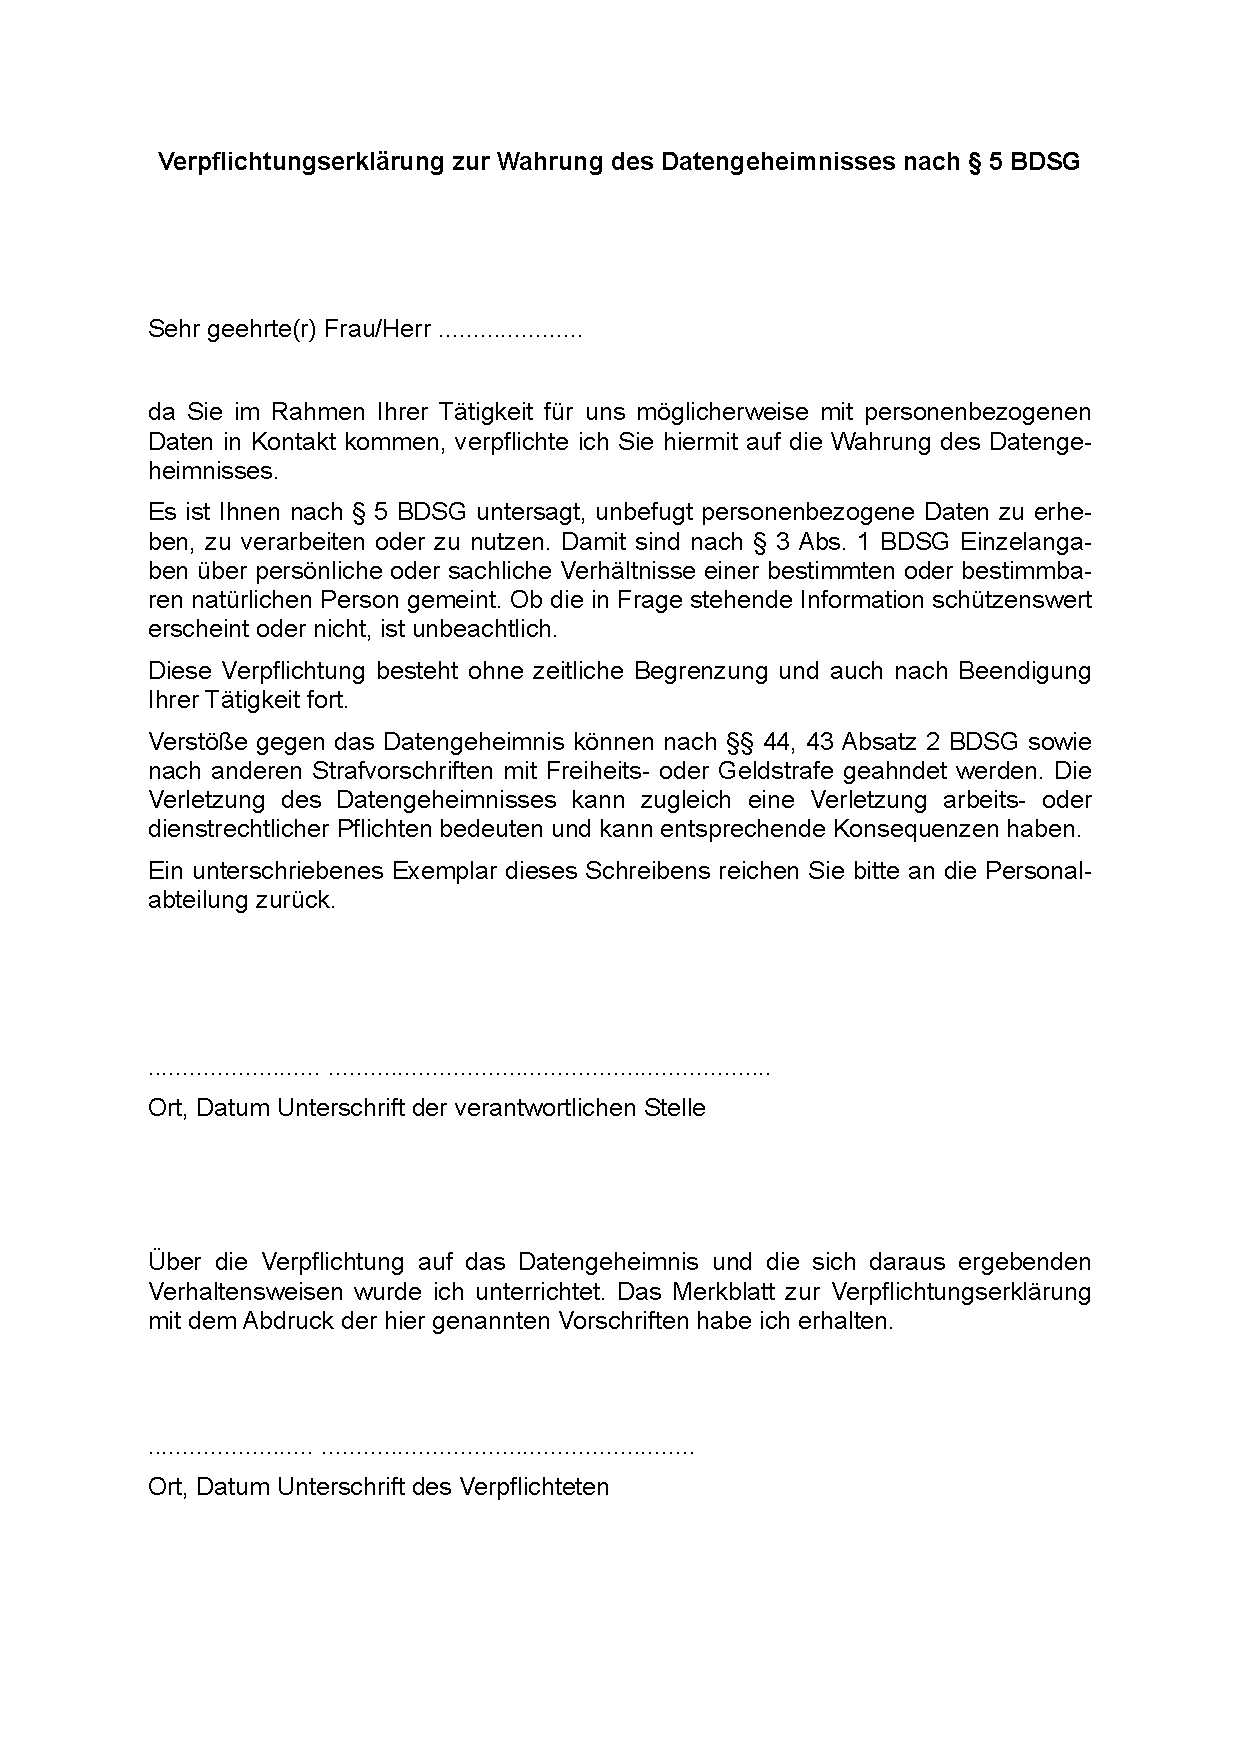
\includegraphics[page=1,width=0.99\textwidth]{./images/datenschutz}
  \end{center}
  \vspace{-40pt}
\end{wrapfigure}

\clearpage

\section{Testfragen}

\begin{wrapfigure}{L}{0.4\textwidth}
  \vspace{-20pt}
  \begin{center}
    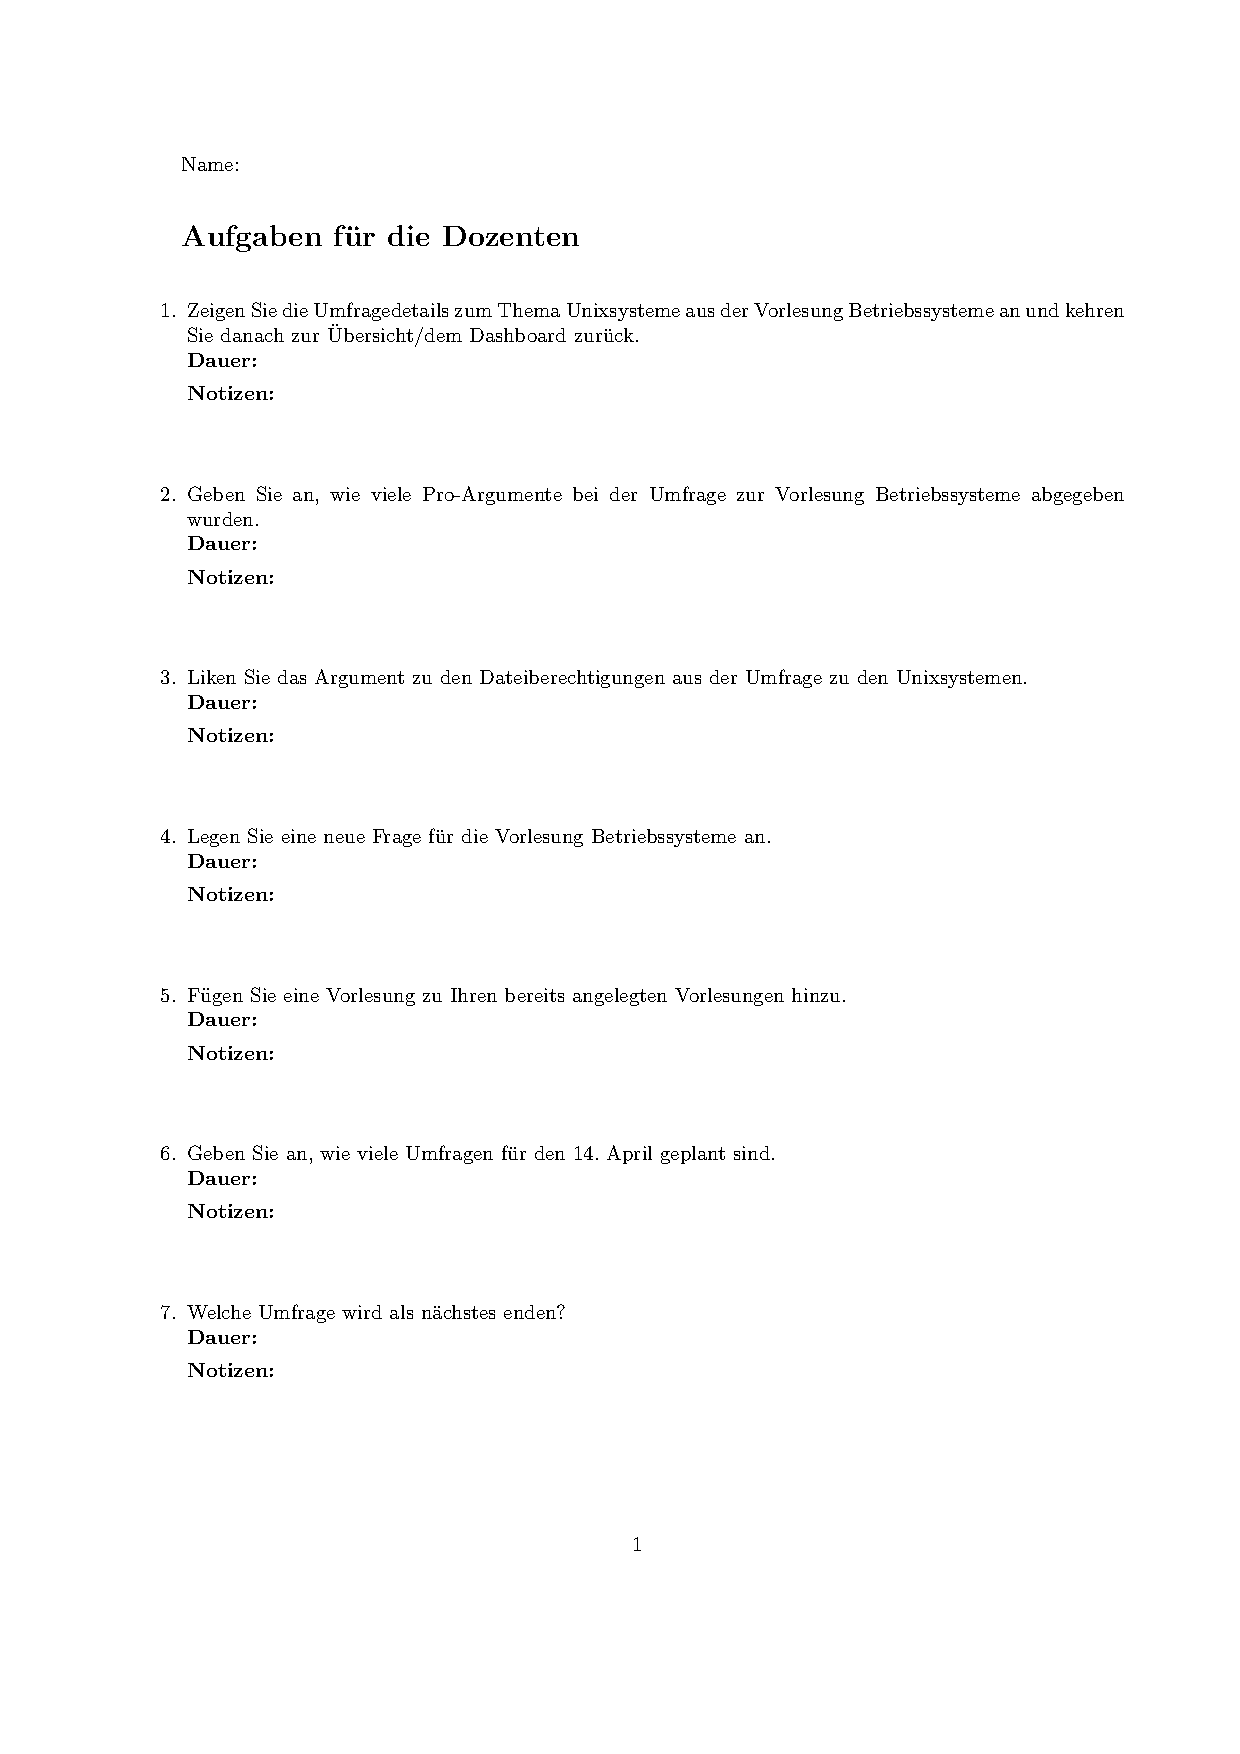
\includegraphics[page=1,width=0.99\textwidth]{./images/probetests}
  \end{center}
  \vspace{-40pt}
\end{wrapfigure}

\begin{wrapfigure}{L}{0.4\textwidth}
  \vspace{-20pt}
  \begin{center}
    \includegraphics[page=2,width=0.99\textwidth]{./images/probetests}
  \end{center}
  \vspace{-40pt}
\end{wrapfigure}

\begin{wrapfigure}{L}{0.4\textwidth}
  \vspace{-20pt}
  \begin{center}
    \includegraphics[page=3,width=0.99\textwidth]{./images/probetests}
  \end{center}
  \vspace{-40pt}
\end{wrapfigure}

\begin{wrapfigure}{L}{0.4\textwidth}
  \vspace{-20pt}
  \begin{center}
    \includegraphics[page=4,width=0.99\textwidth]{./images/probetests}
  \end{center}
  \vspace{-40pt}
\end{wrapfigure}

\clearpage
\section{Nachbefragungs-Formular}
\label{sec:nachbefragung}



\begin{wrapfigure}{L}{0.4\textwidth}
  \vspace{-20pt}
  \begin{center}
    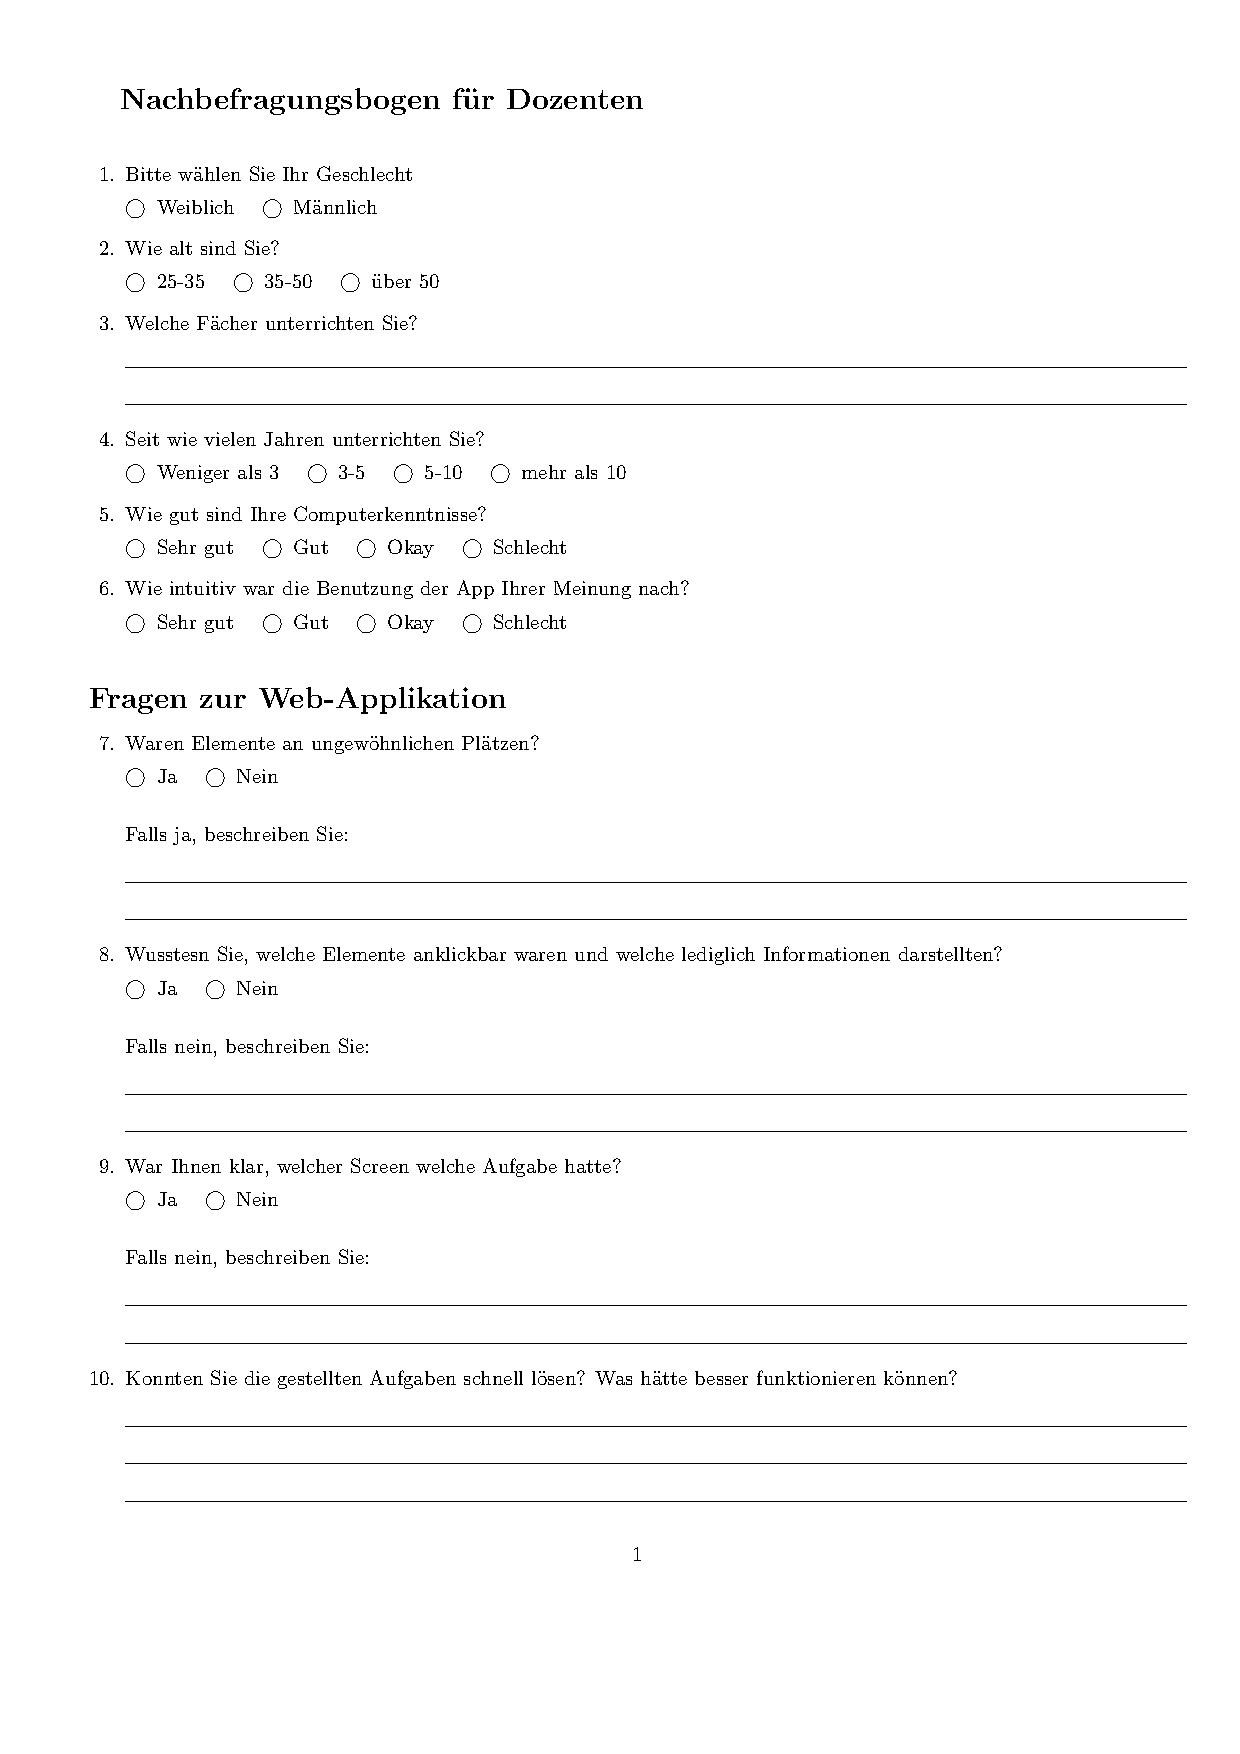
\includegraphics[page=1,width=0.99\textwidth]{./images/dozent}
  \end{center}
  \vspace{-40pt}
\end{wrapfigure}


\begin{wrapfigure}{L}{0.4\textwidth}
  \vspace{-20pt}
  \begin{center}
    \includegraphics[page=2,width=0.99\textwidth]{./images/dozent}
  \end{center}
  \vspace{-40pt}
\end{wrapfigure}


\begin{wrapfigure}{L}{0.4\textwidth}
  \vspace{-20pt}
  \begin{center}
    \includegraphics[page=3,width=0.99\textwidth]{./images/dozent}
  \end{center}
  \vspace{-40pt}
\end{wrapfigure}


\begin{wrapfigure}{L}{0.4\textwidth}
  \vspace{-20pt}
  \begin{center}
    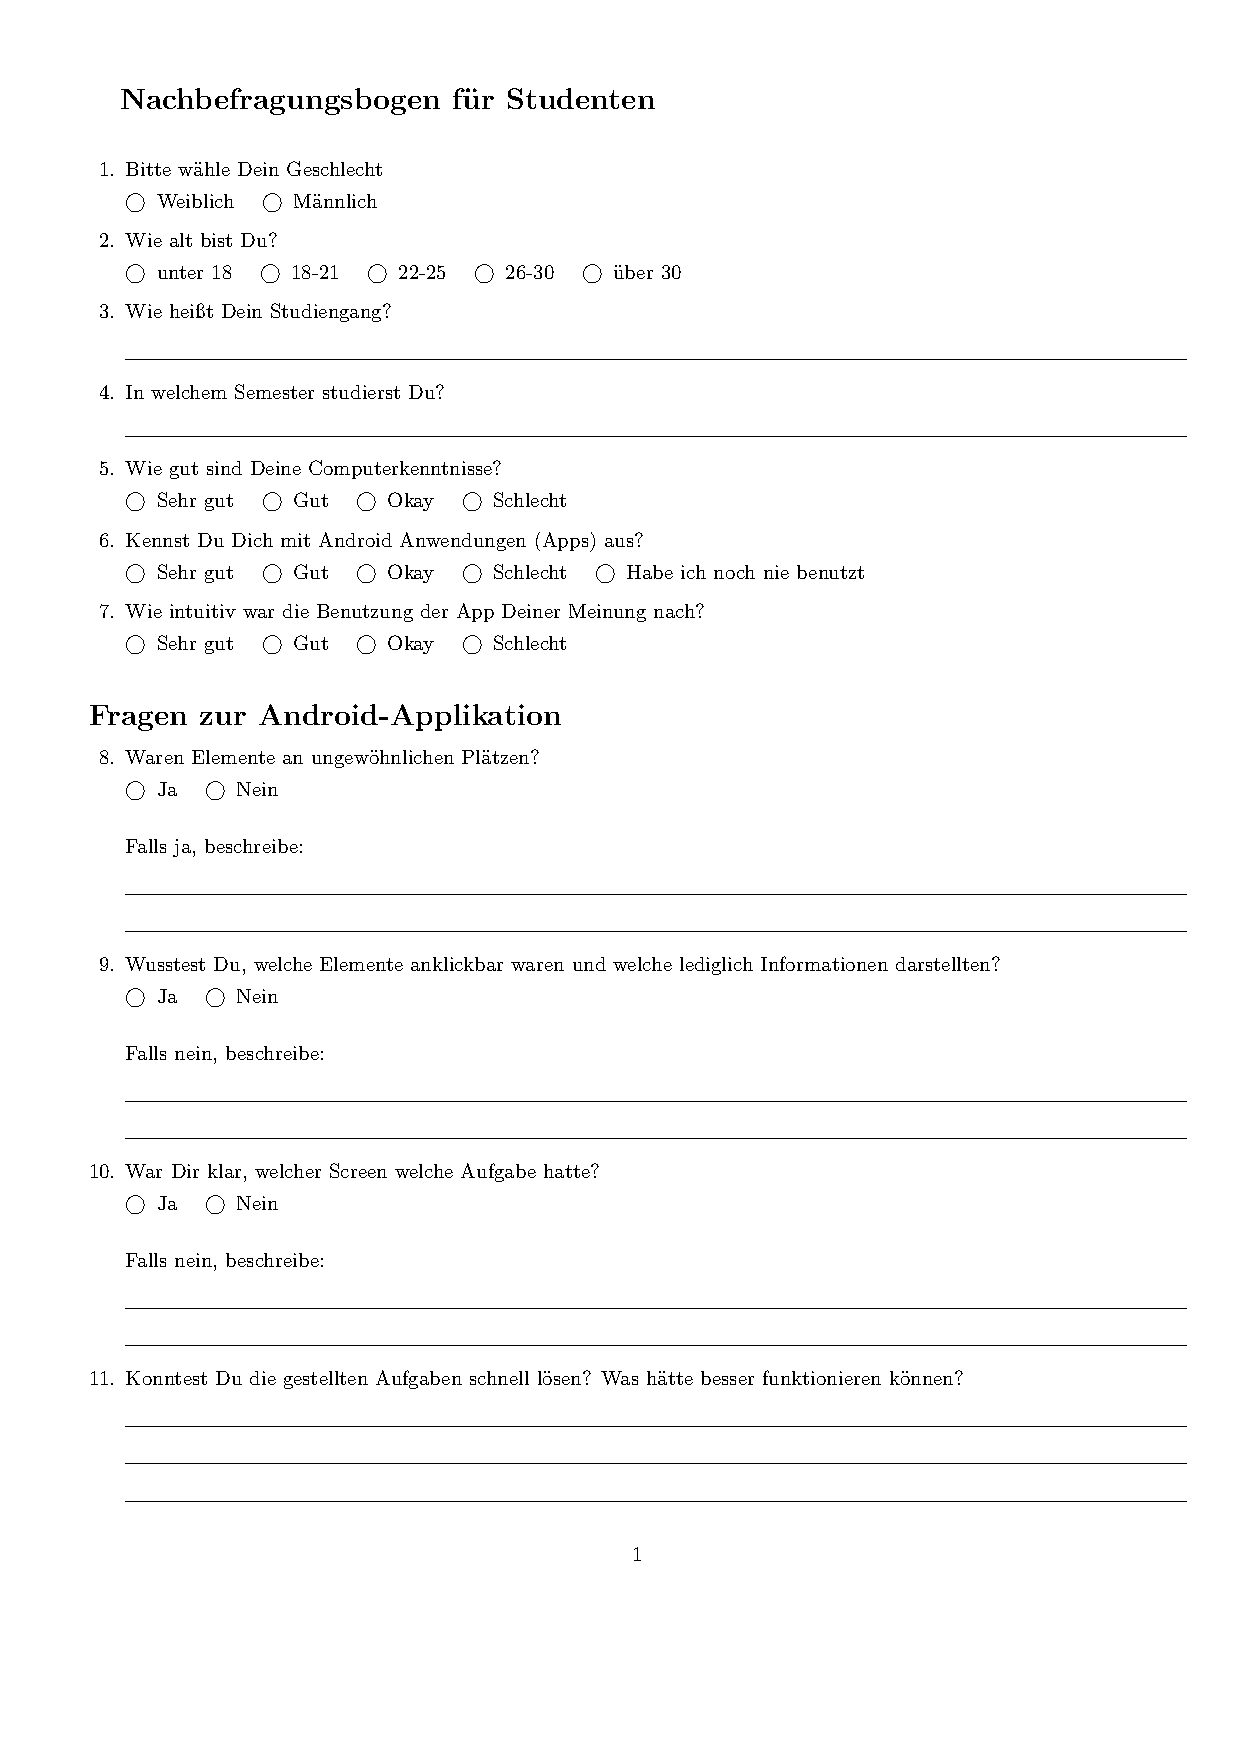
\includegraphics[page=1,width=0.99\textwidth]{./images/student}
  \end{center}
  \vspace{-40pt}
\end{wrapfigure}


\begin{wrapfigure}{L}{0.4\textwidth}
  \vspace{-20pt}
  \begin{center}
    \includegraphics[page=2,width=0.99\textwidth]{./images/student}
  \end{center}
  \vspace{-40pt}
\end{wrapfigure}


\begin{wrapfigure}{L}{0.4\textwidth}
  \vspace{-20pt}
  \begin{center}
    \includegraphics[page=3,width=0.99\textwidth]{./images/student}
  \end{center}
  \vspace{-40pt}
\end{wrapfigure}

\clearpage
\section{Prototypen}
\label{sec:prototypen}

\subsection{Web App}

\begin{wrapfigure}{L}{0.4\textwidth}
  \vspace{-20pt}
  \begin{center}
    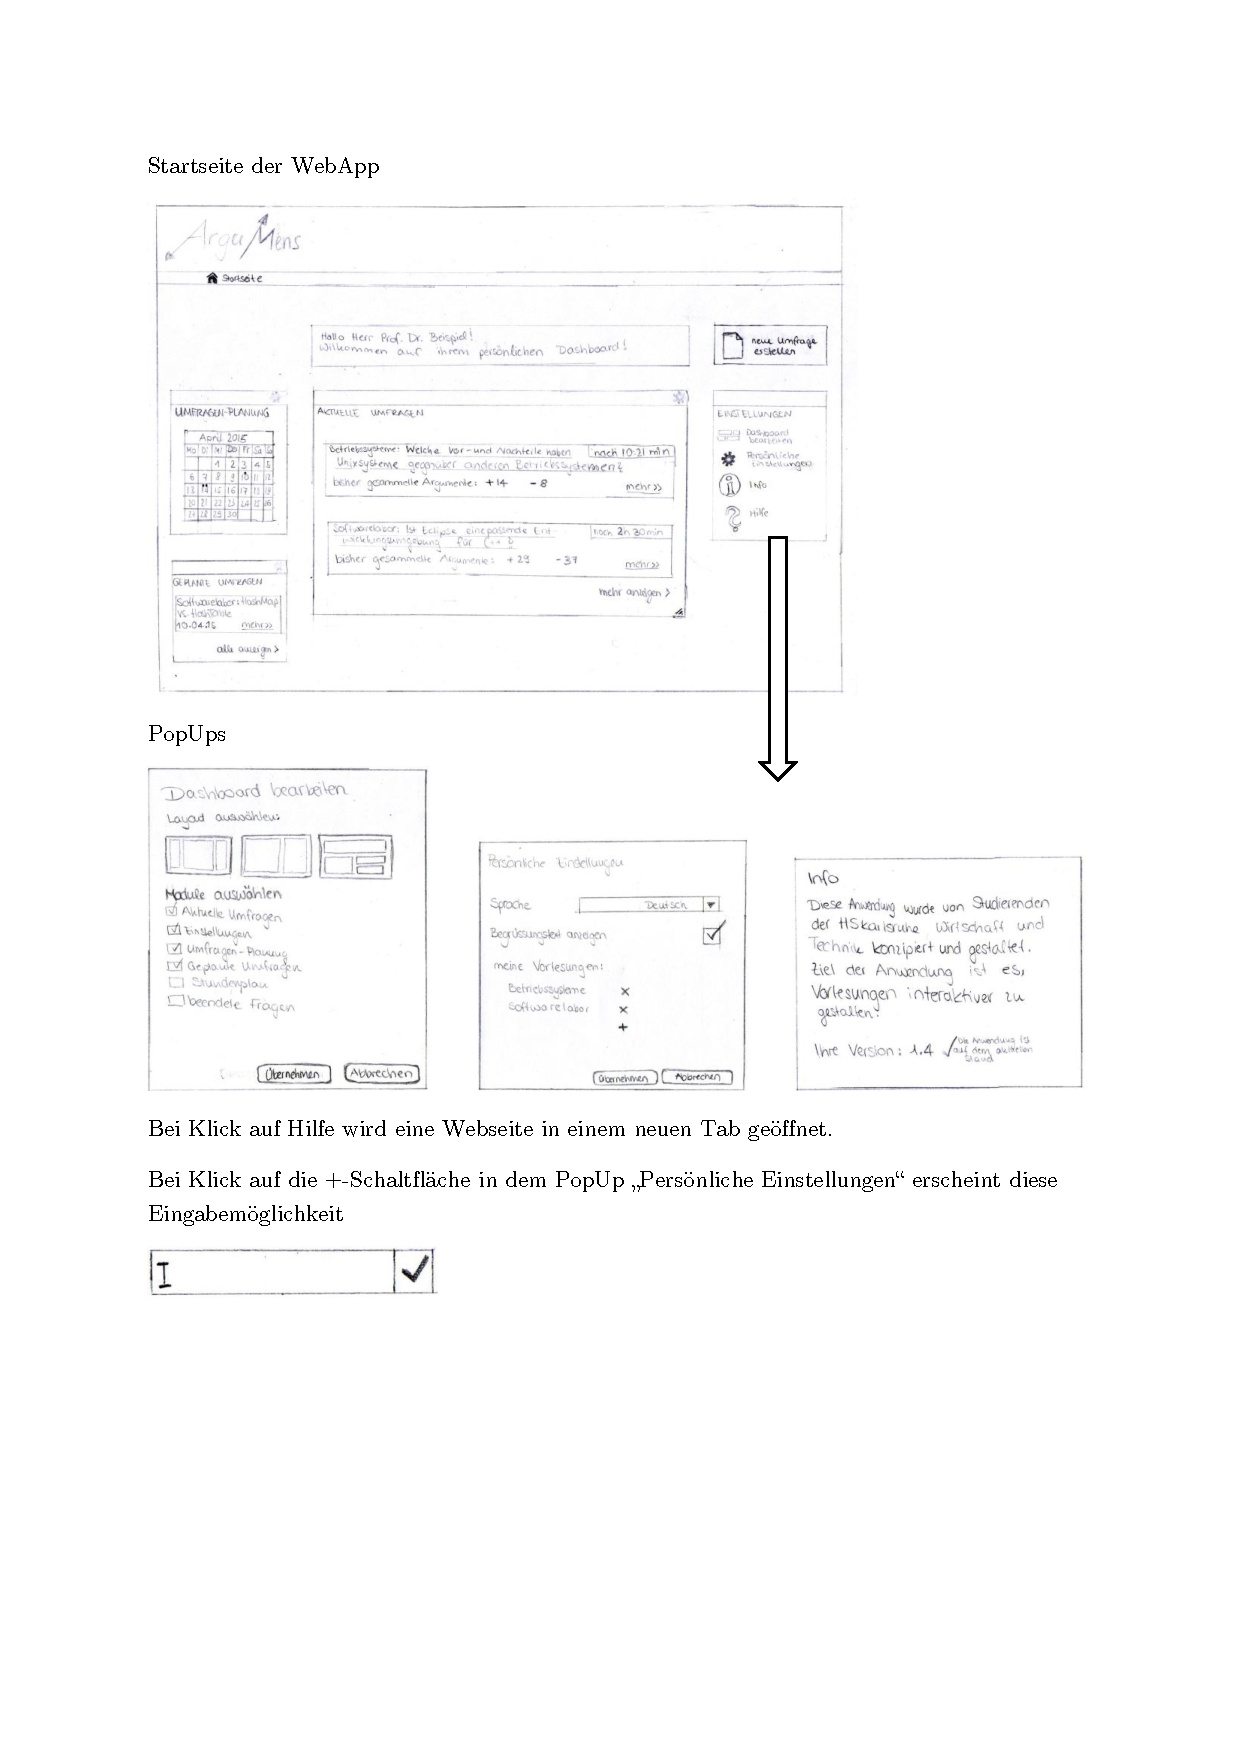
\includegraphics[page=1,width=0.99\textwidth]{./images/prototypWeb}
  \end{center}
  \vspace{-40pt}
\end{wrapfigure}

\begin{wrapfigure}{L}{0.4\textwidth}
  \vspace{-20pt}
  \begin{center}
    \includegraphics[page=2,width=0.99\textwidth]{./images/prototypWeb}
  \end{center}
  \vspace{-40pt}
\end{wrapfigure}

\begin{wrapfigure}{L}{0.4\textwidth}
  \vspace{-20pt}
  \begin{center}
    \includegraphics[page=3,width=0.99\textwidth]{./images/prototypWeb}
  \end{center}
  \vspace{-40pt}
\end{wrapfigure}

\begin{wrapfigure}{L}{0.4\textwidth}
  \vspace{-20pt}
  \begin{center}
    \includegraphics[page=4,width=0.99\textwidth]{./images/prototypWeb}
  \end{center}
  \vspace{-40pt}
\end{wrapfigure}

\begin{wrapfigure}{L}{0.4\textwidth}
  \vspace{-20pt}
  \begin{center}
    \includegraphics[page=5,width=0.99\textwidth]{./images/prototypWeb}
  \end{center}
  \vspace{-40pt}
\end{wrapfigure}

\subsection{Android App}


\begin{wrapfigure}{L}{0.4\textwidth}
  \vspace{-20pt}
  \begin{center}
    \includegraphics[page=1,width=0.99\textwidth]{./images/prototypApp}
  \end{center}
  \vspace{-40pt}
\end{wrapfigure}


\begin{wrapfigure}{L}{0.4\textwidth}
  \vspace{-20pt}
  \begin{center}
    \includegraphics[page=2,width=0.99\textwidth]{./images/prototypApp}
  \end{center}
  \vspace{-40pt}
\end{wrapfigure}


\begin{wrapfigure}{L}{0.4\textwidth}
  \vspace{-20pt}
  \begin{center}
    \includegraphics[page=3,width=0.99\textwidth]{./images/prototypApp}
  \end{center}
  \vspace{-40pt}
\end{wrapfigure}


\begin{wrapfigure}{L}{0.4\textwidth}
  \vspace{-20pt}
  \begin{center}
    \includegraphics[page=4,width=0.99\textwidth]{./images/prototypApp}
  \end{center}
  \vspace{-40pt}
\end{wrapfigure}


\begin{wrapfigure}{L}{0.4\textwidth}
  \vspace{-20pt}
  \begin{center}
    \includegraphics[page=5,width=0.99\textwidth]{./images/prototypApp}
  \end{center}
  \vspace{-40pt}
\end{wrapfigure}


\clearpage
\section{Vorherige Probetests}
\label{sec:probetests}

\paragraph{Rahmenbedingungen}
Wir haben einige Probetests mit verschiedenen Personen durchgeführt. Die Personen stammten zum Teil aus unserer Fakultät und können so als technisch sehr affin eingestuft werden. Des Weiteren haben wir auch Tests mit einem Elternteil durchgeführt, das als mittelmäßig bis wenig technisch affin eingestuft werden kann. Wir haben so zumindest eine kleine Bandbreite verschiedener Personengruppen abdecken können.

Die Tests wurden unter keinerlei Zeitbeschränkung durchgeführt, was uns das Abschätzen der benötigten Zeit für einen konkreten Test erschwert hat. Auch die Testeinleitung wurde teilweise etwas vernachlässigt, da der Großteil der getesteten Personen auch momentan die Vorlesung besucht oder dies in letzten Semestern getan hat. 


\paragraph{Festlegen der Rollenverteilung}
Während der Probetests wurde uns ziemlich schnell klar, wer welche Rolle beim Testen am liebsten und besten einnimmt. So festigte sich unsere Rollenverteilung.

Auch das Sortieren und Ordnen der Prototyp-Bestandteile wurde im Laufe der Probetests immer weiter optimiert, sodass wir jetzt von uns behaupten können, den besten Aufbau für die Testes gefunden zu haben, um Verwirrungen und Zeitverzögerungen zu verhindern.

\paragraph{Ablauf des Tests}
Das Nicht Eingreifen während der Tests stellte sich am Anfang als eine echte Herausforderung dar. Nun sind wir allerdings geübt und es fällt uns nicht mehr so schwer wie zu Beginn. 

Durch unsere Probetests stellten wir einige logische Ungereimtheiten in unseren Aufgabenstellungen fest und bereinigten diese durch eine neue Sortierung. Außerdem verbesserten wir die Formulierungen der Aufgaben, sodass sie für die Probanden leichter zu verstehen wurden. Des Weiteren entfernten wir Aufgabenstellungen, die durch andere schon abgedeckt waren, oder uns unwichtig erschienen.


\paragraph{Technische Ergebnisse}
Durch die Tests haben wir viel gelernt und haben hilfreiche Ideen bekommen, um unsere App intuitiver und besser zu gestalten.

Uns viel auf, dass manche Schaltflächen unpräzise Namen trugen und deshalb die Funktion der Schaltfläche schwerer gefunden wurde. Es wurde oft erst nach besseren Alternativen gesucht, die nicht so schwammig formuliert sind. Da diese aber nicht vorhanden waren fanden die Probanden doch zu den von uns vorgesehenen Schaltflächen, allerdings nicht so intuitiv und schnell wie wir uns das erhofft hatten. Durch eine klarere Formulierung konnten wir positive Ergebnisse im nächsten Probetest feststellen.

Beim Testen mussten wir einsehen, dass gerade Nutzer, die sich im Alltag auf wenig Software beschränken, sich mit manchen Eingabefeldern schwer taten und die dahinter verborgenen Funktionen nicht durchschauten. Unsere Reaktion nach dem Test darauf war, mehr Hilfetexte einzufügen, die dem Benutzer zum Beispiel per Mouse-Over über ein ?-Icon angeboten werden. 

Auch viel uns peinlicherweise auf, dass wir ganze Screens vergessen hatten und konnten diese schnell nachtragen, sodass nun alle Schaltflächen auf einen nachfolgenden Screen verlinken. 
Auch optimierten wir die logische Reihenfolge der Screens und testen verschieden Fälle für einzelne Szenarien.

Als Beispiel dient hier die Funktion „Ein neues Argument anlegen“. Nach erfolgreicher Absendung bekommt der Benutzer eine positive Rückmeldung, dass sein Argument erfolgreich angelegt wurde. Zu Beginn waren wir uns nicht einig, ob der User dabei auf die Umfragen-Detailansicht oder auf die Argument-Detailansicht des soeben erstellten Arguments gelangen soll. Durch die Tests haben wir uns nun für die Argument-Detailansicht entschieden, da der Benutzer so kontrollieren kann, ob er auch alles so eingetragen hat, wie er es möchte. 
Teilweise fehlten bei unseren Popups die Schließen-Schaltflächen, auch diese rüsteten wir nach.

Was unseren Probanden zwar nicht auffiel, uns aber dafür umso mehr war die an manchen Stellen fehlende Konsistenz. Auch hier konnten wir einige Defizite aufarbeiten.

\paragraph{Fazit}
Als Fazit können wir sagen, dass wir bei unseren Tests wenige große Ungereimtheiten aufdecken und viele kleine Verbesserungen anbringen konnten. Diese steigern die Qualität unserer App erheblich. 

Bei unseren Tests wurde uns viel positives, aufmunterndes Feedback entgegengebracht, was uns in unserer Arbeit bestärkt hat.



\section{Testbericht}
\label{sec:testbericht}

\subsection{Im Test erkannte Probleme}
\label{sec:foundproblemes}

Durch den Test der Android-App sind einige Schwächen unseres Prototypen aufgefallen. Besonders hervorzuheben ist hier die Struktur der App.

Beispielsweise ist bereits zu Beginn aufgefallen, dass dem Probanden nicht klar war, was auf dem Homescreen dargestellt wird und was nicht. Wir hatten uns dazu entschlossen, auch bereits abgelaufene Umfragen unter den aktuellen Umfragen aufzulisten, was offensichtlich zur Verwirrung geführt hat. Somit war es für den Probanden nicht klar, dass wir einen separaten Screen für die von ihm abgegebenen Argumente haben, was quasi einem Archiv entspricht.

Als nächstes stellten wir fest, dass der Proband Schwierigkeiten damit hatte die globalen Einstellungen von den Ansichtseinstellungen des Homescreens zu unterscheiden. Gemeint sind hier die Einstellungen zum Ausblenden von bereits abgelaufenen Umfragen und der Sortierung aller Umfragen. Der Button, der dieses Menü aufruft, wurde erst sehr spät gefunden.

Es wurde angemerkt, dass die App in gewissen teilen sehr intuitiv, wie beim Verfassen der Argumente oder dem Aktualisieren der Umfragen, aber auch teilweise aufgrund der verbesserungswürdigen Struktur nicht absolut intuitiv war.
Außerdem muss die Suche verbessert werden um auch abgegebene Argumente zu finden.

Zuletzt viel auf, dass (vor allem auf dem Homescreen) nicht immer klar war, was anklickbar ist und was nicht. Dies wurde offenkundig, als der Proband auf einzelne Teile einer Umfragekachel klickte und eine gewisse Ausgabe erwartete. Dabei sind die Kacheln als Einheit zu sehen.

\subsection{Abgeleitete Verbesserungsvorschläge}
\label{sec:verbesserungsvorschlaege}

Man kann aus denen im Test festgestellten Problemen einige Verbesserungsvorschläge ableiten. Zum Einen sollte man definitiv die Struktur der App überdenken. Der Homescreen sollte die bereits abgelaufenen Umfragen nicht weiter anzeigen, sondern in einen gesonderten Screen auslagern, den man als Archiv bezeichnen kann. Hierbei ist dann noch wichtig, dass eine Differenzierung der bereits abgelaufenen Umfragen und der von dem Benutzer abgegebenen Argumente zu allen (auch abgelaufenen) Umfragen notwendig ist. Wie man diese Teile am besten trennt, müsste durch weitere Tests herausgefunden werden. Dadurch, dass diese Funktionalität jedoch vermutlich nur selten genutzt wird und daher keine wichtige Funktion ist, sollte man diese Screens in das Slide-In Menü integrieren, da dieses Menü primär genutzt wird, wenn man erweiterte Funktionen benötigt.

Außerdem sollte man die Sortierung der Umfragen in die bereits existierenden Einstellungen auslagern, da die App somit noch simpler wird.

Zuletzt muss man, wie oben angemerkt, die Suche verbessern und verfeinern und die anklickbaren Elemente grafisch verbessern.

\subsection{Kritik und Bewertung des Tests}
\label{sec:kritik}

Beim Test unseres Prototypen sind uns einige Dinge aufgefallen, die primär konzeptioneller Natur waren. Es hat bereits damit angefangen, dass wir durch technische Probleme nicht alle Dokumente ausdrucken konnten und somit dann auch zu spät zu dem verabredeten Test gekommen sind. Daraus entstand dann eine entsprechend gestresste Situation, die man durch bessere Planung hätte umgehen können. 
Nachdem wir dann alles für den Test gerichtet hatten fiel relativ schnell auf, dass wir unsere App zu ausführlich testen wollten und dass wir uns nicht auf spezielle Fälle fokussierten. Wir wollten sowohl die Webapplikation, als auch die Android App testen und hatten dafür sehr viele Testfälle vorbereitet, was auch dem Testleiter bewusst war. Daraus resultierte, dass die Testvorbesprechung viel zu kurz kam und eventuelle Fragen eventuell nicht geklärt wurden.
Beim eigentlichen Test haben wir dann festgestellt, dass die eigentlichen Funktionen erst viel zu spät dran kamen, so hatten wir als ersten Fall gefragt, wie man Einstellungen ändert und das Archiv findet und daraus Informationen ableitet. Es wäre an dieser Stelle wesentlich sinnvoller gewesen, wenn man zuerst die Abfrage von Informationen zu den existierenden Umfragen gefordert hätte, da sich der Proband dann auch schneller an den strukturellen Aufbau der App hätte gewöhnen können und somit die Aufgaben schneller hätte lösen können. Durch unsere Fragen verwirrten wir den Probanden jedoch massiv, was während dem Test alles andere als förderlich war.

Wie bereits angesprochen, haben wir die Testdauer unterschätzt, so kam es dazu, dass wir Testaufgaben überspringen mussten und der Prototyp für die Webapp überhaupt nicht getestet wurde. In Zukunft ist eine bessere Abschätzung des Verlaufs von essenzieller Bedeutung.

Es fiel zudem auf, dass der Testleiter während des Tests die Aktionen des Probanden in einigen Fällen durch seine Aussagen bewertete. Dies sollte, wie in der Anfangsbesprechung auch gefordert, vermieden werden.

Auch wenn nicht alles absolut perfekt funktioniert hat, kann man festhalten, dass wir durch die gemachten Fehler viel gelernt haben, was man in Zukunft vermeiden kann.

\clearpage